\graphicspath{{Chapter_2_-_Notions_of_thermodynamics/Images/}}
\chapter{Notions of the thermodynamics}
\quad\, In the introduction, it has been introduced many times the concept and the used of the Brayton cycle. As explained, this concept has been applied for many usages, including electricity production and aircraft propulsion which are the most common and known applications. It has been exposed that from the invention proposed by George Brayton in the end of the 19th century, the technology did really evolve.

Indeed, while the Brayton cycle engine first appears as a  piston engine where the compression, combustion and expansion occurs in the same enclosure, Nowadays 
the process is shared between at least three components (namely the compressor, the turbine and the combustion chamber).

However, what the previous did not cover were the keys notions to understand how theses components behave. Those notions, which will be used during this work, need to be defined and explained to allows to the common person to understand this writing without possessing those knowledge a priory. 
This problematic will be covered by this chapter, which will introduce step-by-step those notions.

\section{Fundamental notions}
\quad\, As mention in the lead-in of this chapter, the first sections of this report will entirely be devoted to the bringing in of the required knowledge for the understanding of the full report.

Starting from very fundamental notions, those will allow to explain more complex concept that will be applied in this work.
\newpage
\subsection{Open/closed system}\label{sect:C2_Sys}
\quad\,  The thermodynamic is a science that "studies the exchange of energy between a system and its environment or surrounding" \cite{thermoApp_1}.

The system is defined as being the area of the space selected for the study. Between the system and the environment lies the boundary. This boundary can either be real or fictitious and, can be static or mobile.

When the system is characterized, it has to be established if it is an open or a closed system.
The open systems are ones where an arbitrary control volume well demarcated in the space is studied. For these systems, matter and energy is exchanged with the surrounding as heat or work. Typical examples are combustion chamber, heat-exchanger, turbomachines, piping,...

On the other hand, the closed systems does not exchange matter with the environment. Indeed, 
for those systems a control mass well delimited in the space is studied. Therefore, the exchange of mass with the environment is prohibited for this category of system. 

\subsection{State functions and variables}\label{sect:C2_State}
\quad\, Let considered a system as defined in the previous section. The state functions are defined as "a property of the system that only depend on its current state". These functions are independent of the past of the system and describe the equilibrium state of the system.

When the state functions can be measured (directly or indirectly), these are called state variables. For example, the pressure $P$, the temperature $T$ or the volume $Vol$ are state variables.

It can be shown that the equilibrium state of a system can be described by those three variables. Also, among $P$, $T$ and $Vol$, only two of them are independent. This means that a state relation defined as \textbf{F}($P$, $T$, $Vol$) = 0.

For the ideal gas, this relation is
\begin{align}
\setstretch{1}
P\cdot Vol &= m\cdot\frac{R}{MM}\cdot T\nonumber\\
P\cdot vol &= r\cdot T\label{eq:C2_GP}    
\end{align}
where \textit{m} is the quantity of matter (in kg), $R$ is the universal gas constant (8.314 J/mole/K\footnote{Where K is the degree Kelvin and is scaled as 273.15\degree K = 0\degree C}), $vol$ the specific volume (in m$^3$/kg) and $MM$ is the molar mass (in kg/mole\footnote{Where 1 mole correspond to $\sim 6\cdot 10^{23}$ elementary entities (atoms, molecules,...)}) of the system.
\newpage
\subsection{Energy}\label{sect:C2_Ener}
\quad\, In the subsection \ref{sect:C2_Sys}, the notion of energy has been mentioned without characterizing it before hand. From the first principle of the thermodynamic, it is stated that the energy cannot be created nor destroyed. Therefore, it can only be converted an can exist into multiple forms (thermal, mechanical, electrical,...)\cite{thermoApp_2}. The unit of the energy is the Joule (J), and the sum of all the energies in a system is called the total energy $E$.

The energy is a state variable. This means that this quantity allows to characterize the state of the system. When considering the energy, its absolute value is not something that is defined. Instead, the energy is always computed as compared with a reference point.

Thus, considering the variation of the total energy from a state \textbf{1} to a state \textbf{2}, it is obtained
\begin{align}
\setstretch{1}
    \Delta E &= \Delta U + \Delta KE + \Delta PE \label{eq:C2_E}\\
    \text{with } \Delta U  &= U_2 - U_1 =  m\cdot(u_2 - u_1) \text{: Variation of the internal energy}\nonumber\\
                 \Delta KE &= \frac{1}{2}m\cdot(v^2_2 - v^2_1)\text{: Variation of the kinetic energy}\nonumber\\
                 \Delta PE &= m\cdot g\cdot(z_2 - z_1)\text{: Variation of the potential energy}\nonumber
\end{align} 
where $z$ is the altitude of the system position, $v$ is the velocity of the fluid and $U$, the internal energy, is the sum of all the "microscopic" energy within the system. The $u$ in lowercase corresponds to the specific internal energy and its unit is in J/kg.

As said in the subsection \ref{sect:C2_Sys}, any system will exchange energy with the surrounding as heat and/or work. The heat is defined as "the form of energy which is exchanged between the system and its environment when there is a gradient of temperature between these two entities". As the heat is always referred as a flux between two bodies, the phenomena is called heat transfer. The heat transfer can be realized by
\begin{itemize}
\setstretch{1}
    \item Conduction: Heat transfer through a non flowing material due to the interaction of "molecular scale energy carriers within the material"\cite{GregoryNellis2015}
    \item Convection: More complex conduction when considering a flowing fluid.
    \item Radiation: The heat is transferred as electromagnetic waves.
\end{itemize}
The heat transfer is denoted $Q$. A system that does not exchange heat with the surrounding is called \textbf{adiabatic}.

Aside the heat transfer, the system also can exchange energy by producing a work. The Work $W$ is "the form of energy exchanged associated to a force applied over a certain distance". The work is exchanged if the force applied on the system creates a displacement of its boundary. The power is defined as the work per unit of time (in Watt or W).

Both the heat and the work are called "path functions" because they are associated to the evolution of a system and not to the state of this system. Thus, these are not thermodynamic variables (like the temperature or the pressure).

\subsubsection{Energy balance}
\quad\, It has been previously mentioned several mechanisms to exchange energy from the system to its environment. Aside from the heat transfer and the work transfer, the energy can also be exchange using mass transfer. Indeed, if the considered system is open, the mass entering and exiting the system will convey energy.

To recall the first principle of the thermodynamic, the energy cannot be created or destroyed. Based on the statement, the energy balance of the system is given by the following generic formulation (\ref{eq:C2_EB}).
\begin{equation}
\setstretch{1}
    E_{in} - E_{out} = (Q_{in} - Q_{out}) + (W_{in} - W_{out}) + (E_{mass,in} - E_{mass,out}) = \Delta E_{system} \label{eq:C2_EB}
\end{equation}
with $E_{mass}$ the energy convey by the mass entering/exiting the system.

It is possible to write a temporal formulation (\ref{eq:C2_PB}) of the energy balance named \textbf{power balance}.  
\begin{equation}
\setstretch{1}
    \dot{E}_{in} - \dot{E}_{out} = (\dot{Q}_{in} - \dot{Q}_{out}) + (\dot{W}_{in} - \dot{W}_{out}) + (\dot{E}_{mass,in} - \dot{E}_{mass,out}) = \frac{dE_{system}}{dt} \label{eq:C2_PB}
\end{equation}
where $\frac{dE_{system}}{dt}=0$ when considering a system for which the variation of energy does not vary in the time.

\subsubsection{Energy conservation efficiency}
\quad\, When the system is transferring or converting energy, it is often interesting to quantified the quality of this transfer/conversion. the efficiency is defined to provide this quantification and its definition is the
$\frac{\text{Desired ouptut}}{\text{Required input}}$. For example, a water electric heater with a efficiency of 90\% is a system such that 90\% of the electrical energy consumed is converted in thermal energy.  

Considering the combustion of a fuel, the combustion efficiency is defined as the ratio
$$ \frac{\dot{Q}}{\dot{m}_{fuel}\cdot HV_{fuel}}$$
where $\dot{m}$  and $HV_{fuel}$ is the mass flow and the heating value of the fuel injected into the combustion chamber.
\section{Principles of the thermodynamic}
\quad\, The previous section did introduce many concepts to start analyzing a thermodynamic system submitted to diverse transformations. Among those, the notion of state variables defining the equilibrium state of such system has been defined. This section will used the first and second principles of the thermodynamic to introduce some state variables that are used when studying a thermodynamic cycle.

\subsection{Enthalpy}
\quad\, Considering a closed system, the third term of the energy balance given in the relation(\ref{eq:C2_EB}) is nullified. Thus, the variation of the total energy from a state \textbf{1} to a state \textbf{2} is equal to
\begin{equation}
\setstretch{1}
E_{2} - E_{1} = Q_{1-2} - W_{1-2} = m\cdot\left(u_2 - u_1\right) + \frac{1}{2}m\cdot\left(v^2_2 - v^2_1\right) + m\cdot g\cdot\left(z_2 - z1\right)\citep{Dewallef2019} \label{eq:C2_EBC}
\end{equation}
Let's note that the terms of kinetic and potential energy are often negligible compared to the internal energy.  

The relation \ref{eq:C2_EBC} can be adapted to be applied for the open system by introducing an accumulation term $\Delta E_{cv}$. This correction allows the following reformulation (\ref{eq:C2_EBO}) of the energy balance.
\begin{equation}
\setstretch{1}
Q_{1-2} - W_{1-2} - E_{2} - E_{1} = \Delta E_{cv}\label{eq:C2_EBO}
\end{equation}

\begin{figure}[h]
\centering
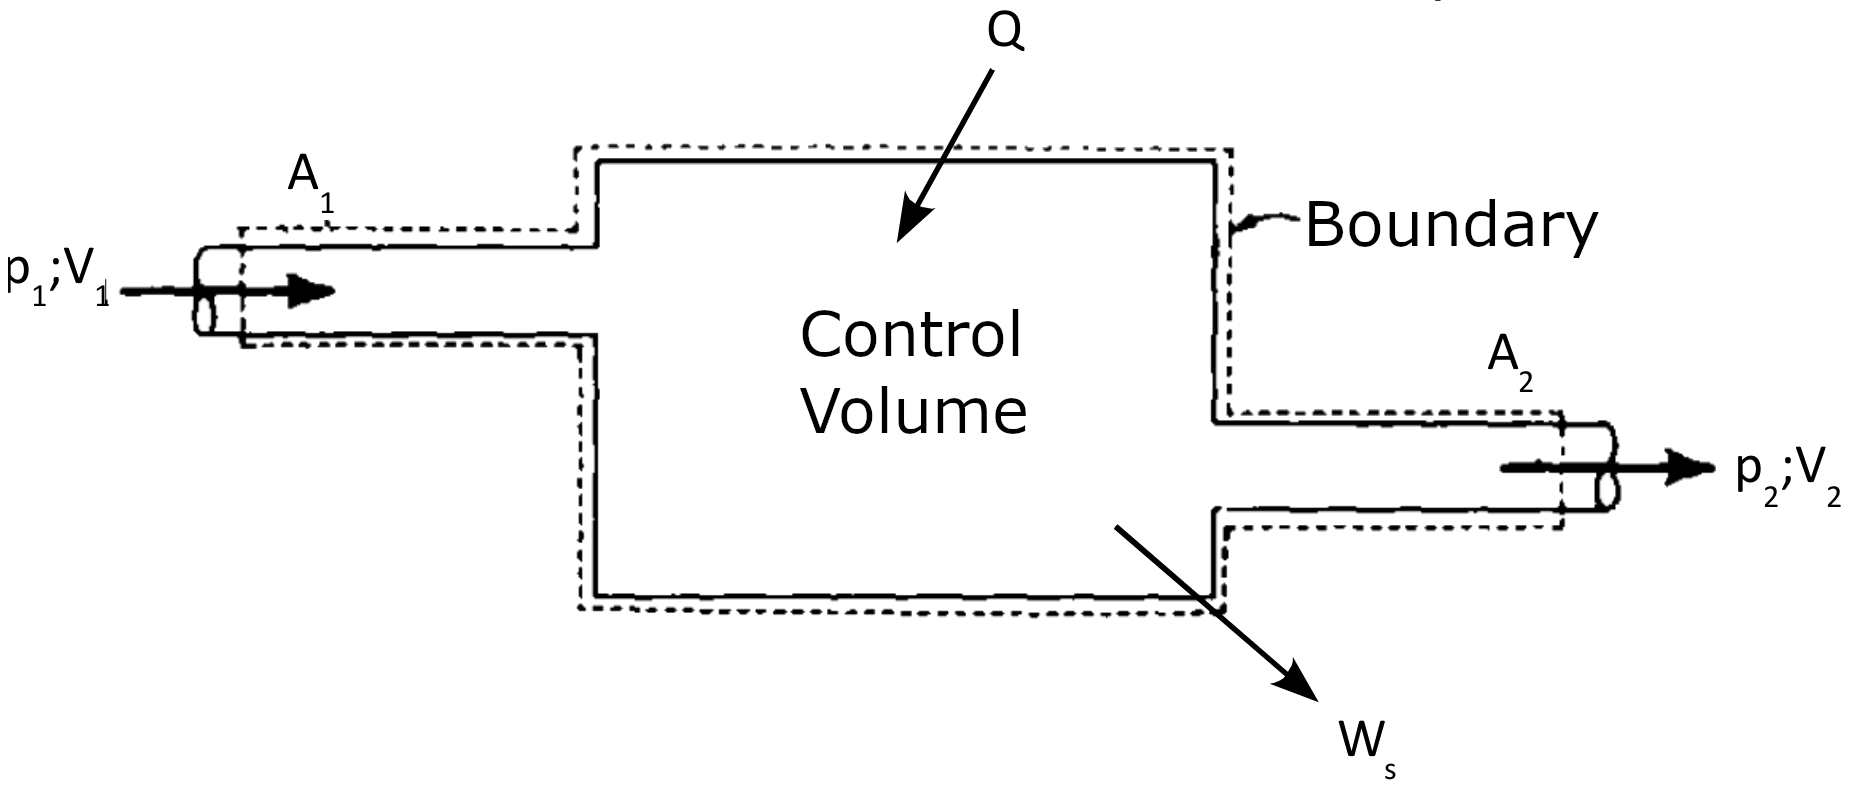
\includegraphics[width=0.7\textwidth]{control_volume.png}
\caption{System control volume \cite{Dewallef2019}}
\label{fig:C2_VC}
\end{figure}

The Figure \ref{fig:C2_VC} depicts an open system with an entry and exit area $A_1$ and $A_2$ respectively. Posing that the work $W$ is equal to 
\begin{equation}
\setstretch{1}
W = P_2\cdot A_2\cdot v_2\cdot \Delta t - P_1\cdot A_1\cdot v_1\cdot \Delta t + W_s
\end{equation}      
where $P_1$ (resp. $P_2$) and $V_1$ (resp. $V_2$) are the pressure and the velocity at \textbf{1} (resp. \textbf{2}).

By neglecting the variation of the kinetic and potential energy, the energy balance is after some mathematical operations as given in the relation \ref{eq:C2_EBH}
\begin{equation}
\setstretch{1}
q - w_s = u_2 +P_2\cdot vol_2 - u_1 - P_1\cdot vol_1 = h_2 - h_1\label{eq:C2_EBH}
\end{equation}
where $q$, $w_s$, and $h$ are respectively the specific work, heat and \textbf{enthalpy} (in J/kg).  
For the case of an ideal gas, the enthalpy and the internal energy only depend on the temperature $T$. Indeed, taking the equation (\ref{eq:C2_GP}), the relation (\ref{eq:C2_h}) can easily be deduced.
\begin{equation}
\setstretch{1}
h = u(T) + Pvol = u(T) + rT \label{eq:C2_h}
\end{equation}
\subsection{Specific heat}
\quad\, The previous subsection was meant to define the enthalpy. This state variable is used in place of the internal energy when dealing with open system.\\

An other quantity that is useful for system study is the \textbf{specific heat}. This state variable is defined as the required energy to increase of 1\degree C the temperature of 1kg of a substance. 
 
The required heat to produce this effect depends on the ways the transformation takes place. 
If it is done under constant volume constraint, it is called specific heat at constant volume and denoted $c_v$. 

If the transformation is performed at constant pressure, the symbol associated to the specific heat is $c_p$.
It is worth to note that the specific heat at constant pressure is always higher than the $c_v$. When performing the transformation a constant pressure, the gas expands against the external pressure. This means that the gas does work and, this is the reason behind the greater value of the supplied heat when dealing with a transformation at constant pressure. 

It had been shown that for an ideal gas, the variation of the internal energy can be linked to the specific heat at constant volume as written in the relation (\ref{eq:C2_UC}).
\begin{equation}
\setstretch{1}
du = c_vdT \rightarrow u_2 - u_1 = \int_{T_1}^{T_2} c_vdT\label{eq:C2_UC}
\end{equation} 
Similarly, the variation of the enthalpy can be expressed using the specific at constant pressure.

\begin{equation}
\setstretch{1}
dh = c_pdT \rightarrow h_2 - h_1 = \int_{T_1}^{T_2} c_pdT\label{eq:C2_UP}
\end{equation} 

These two relations, with the equality (\ref{eq:C2_h}), provide the required tools to express the gas constant $r$ as a function of the temperature only. 
\begin{equation}
\setstretch{1}
r = c_p - c_v \label{eq:C2_r}
\end{equation}

Aside the gas constant, the specific heat ratio $k$ (\ref{eq:C2_k}) is also a useful variable to be computed.
\begin{equation}
\setstretch{1}
k = \frac{c_p}{c_v} \label{eq:C2_k}
\end{equation}

\subsection{Carnot cycle}
\quad\, The previous subsections used the first principle of the thermodynamic to deduce two useful state variables, namely the enthalpy and the specific heat.

Now, let's move aside those notions and let consider the case where the transformation applied to a system is reversible. A necessary condition for the reversibility is that the transformation has to be done in quasi-equilibrium. This implies that if the transformation is reversed, the system goes back to its initial state.


\begin{figure}[h]
\centering
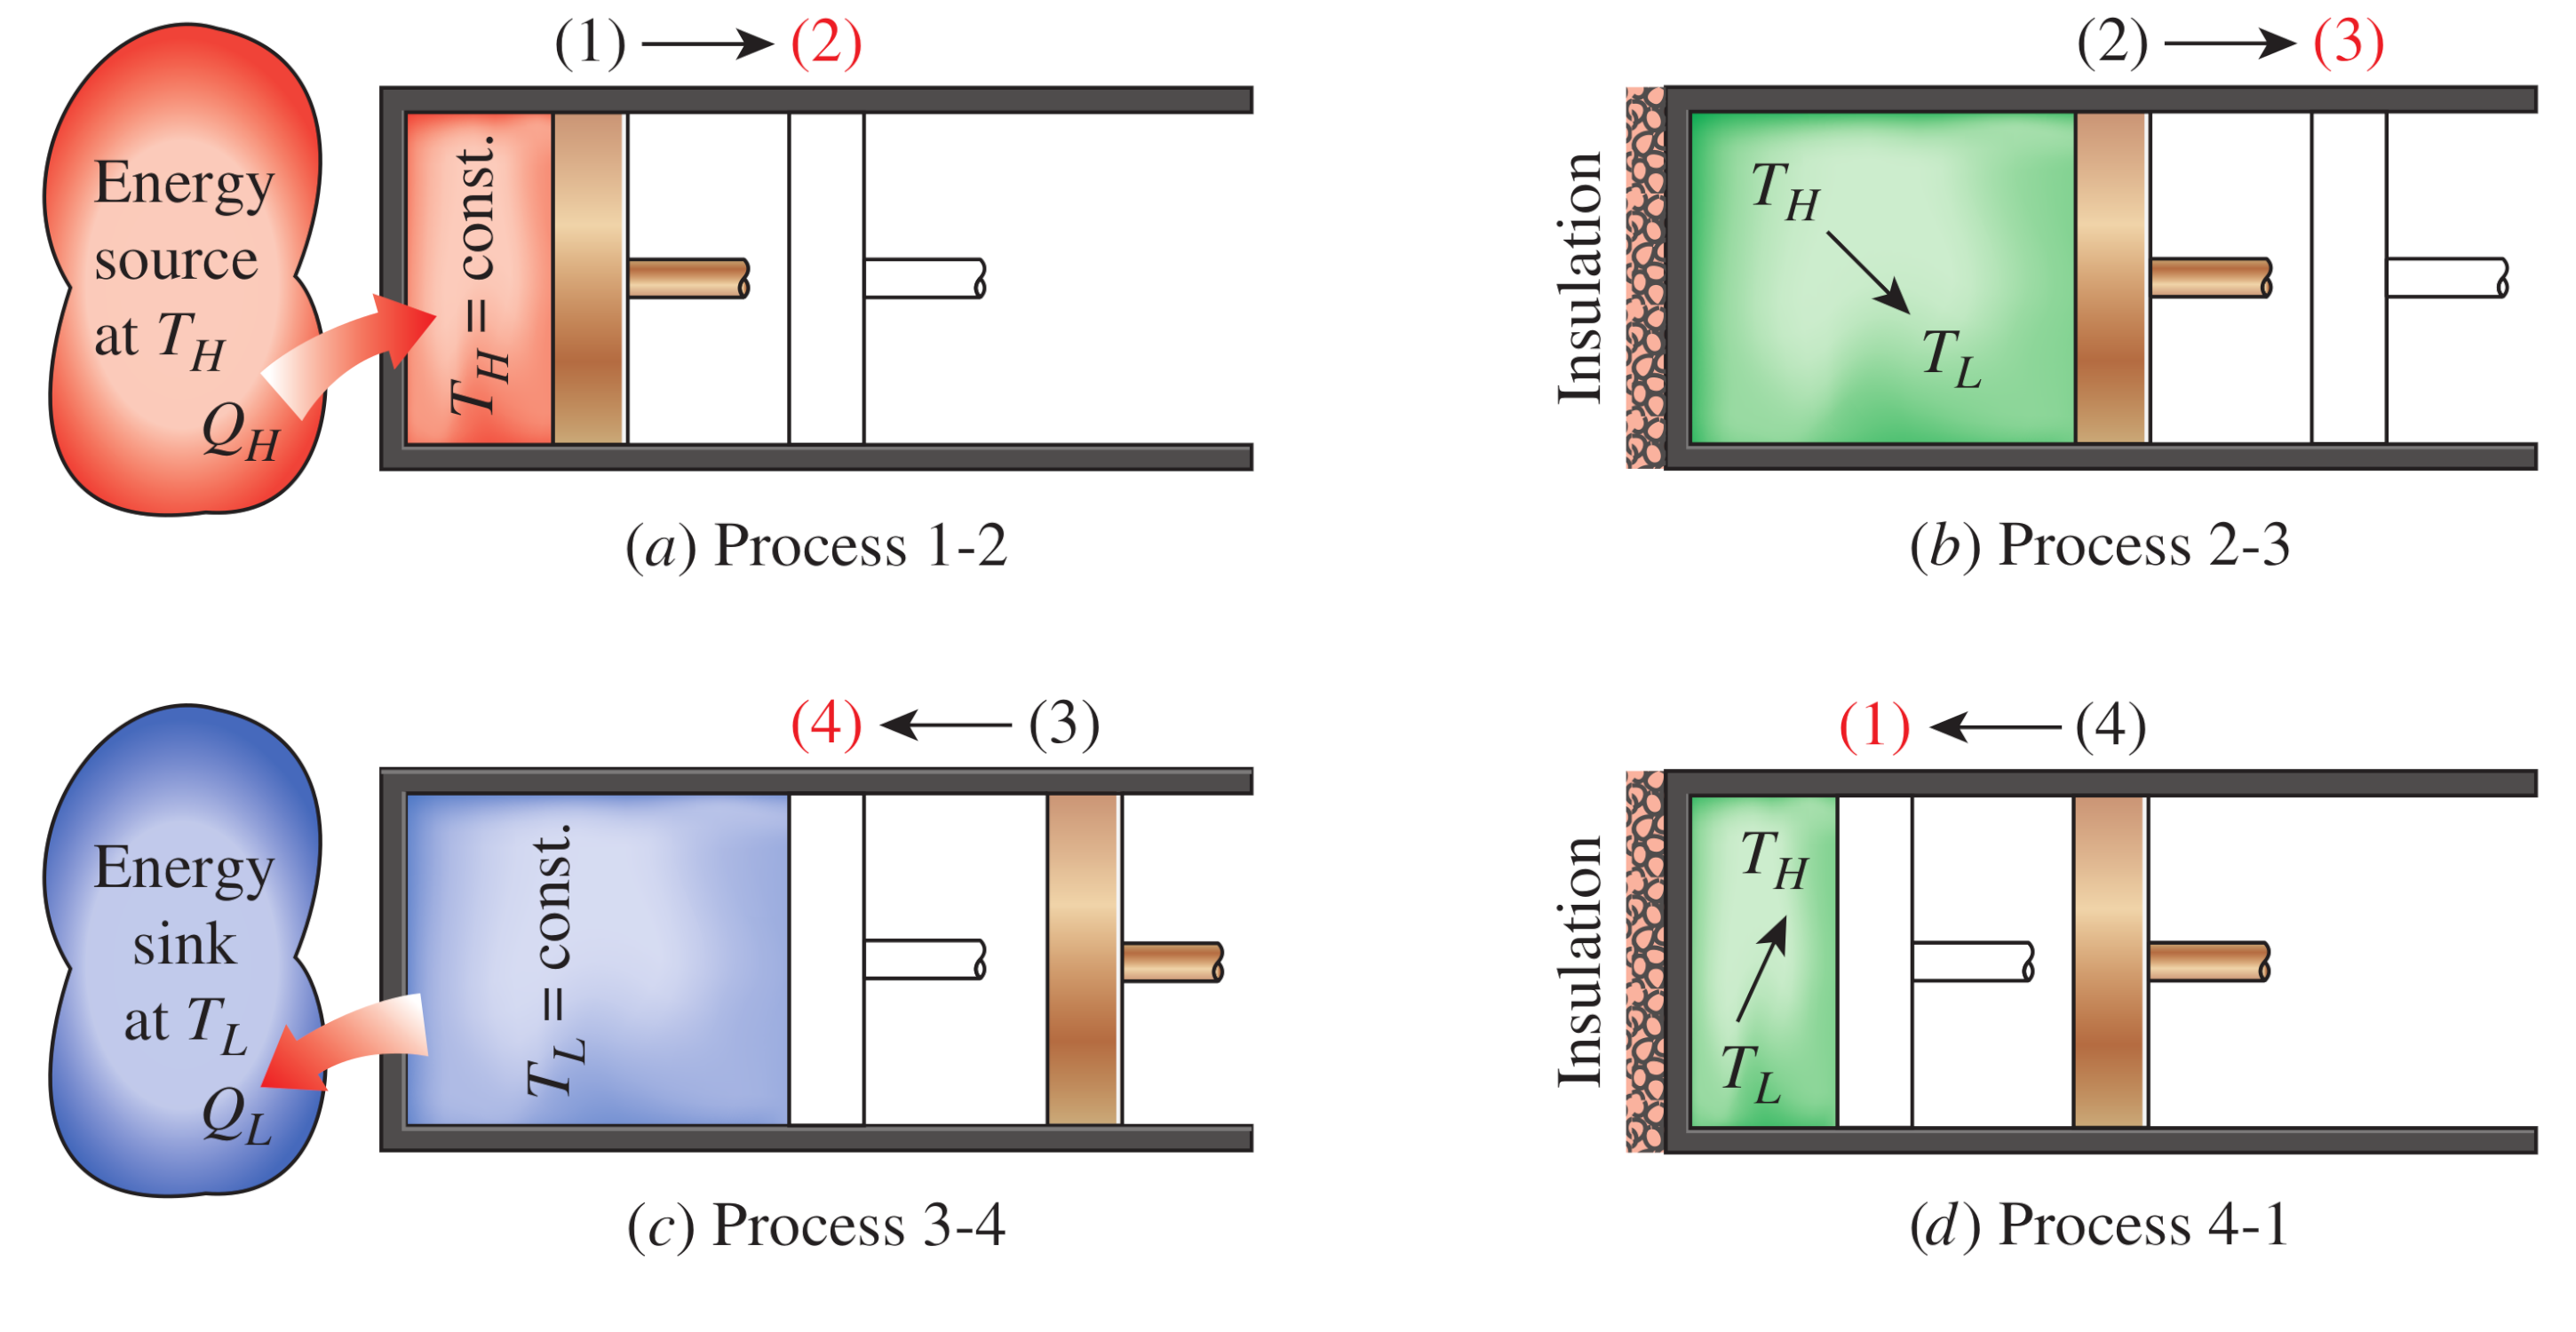
\includegraphics[width=0.7\textwidth]{Carnot_schema.png}
\caption{Carnot cycle - Schematic \cite{2015}}
\label{fig:C2_Carnot}
\end{figure}
The Carnot cycle is a thermodynamic cycle composed of 4 reversible transformations illustrated on Figure \ref{fig:C2_Carnot}. The transformations are defined as follows.

\begin{itemize}
\setstretch{1}
\item \textbf{1} to \textbf{2} (Figure \ref{fig:C2_Carnot}a): Reversible isotherm expansion with a heat transfer $Q_H$ from the environment to the system
\item \textbf{2} to \textbf{3} (Figure \ref{fig:C2_Carnot}b): Reversible  adiabatic expansion
\item \textbf{3} to \textbf{4} (Figure \ref{fig:C2_Carnot}c): Reversible isotherm compression with a heat transfer $Q_L$ from the system to the environment
\item \textbf{4} to \textbf{1} (Figure \ref{fig:C2_Carnot}d): Reversible adiabatic compression
\end{itemize}
For visual representation, this cycle has been represented in the PV diagram \ref{fig:C2_CarnotPV} where the different transformations are well exposed.
\begin{figure}[h]
\centering
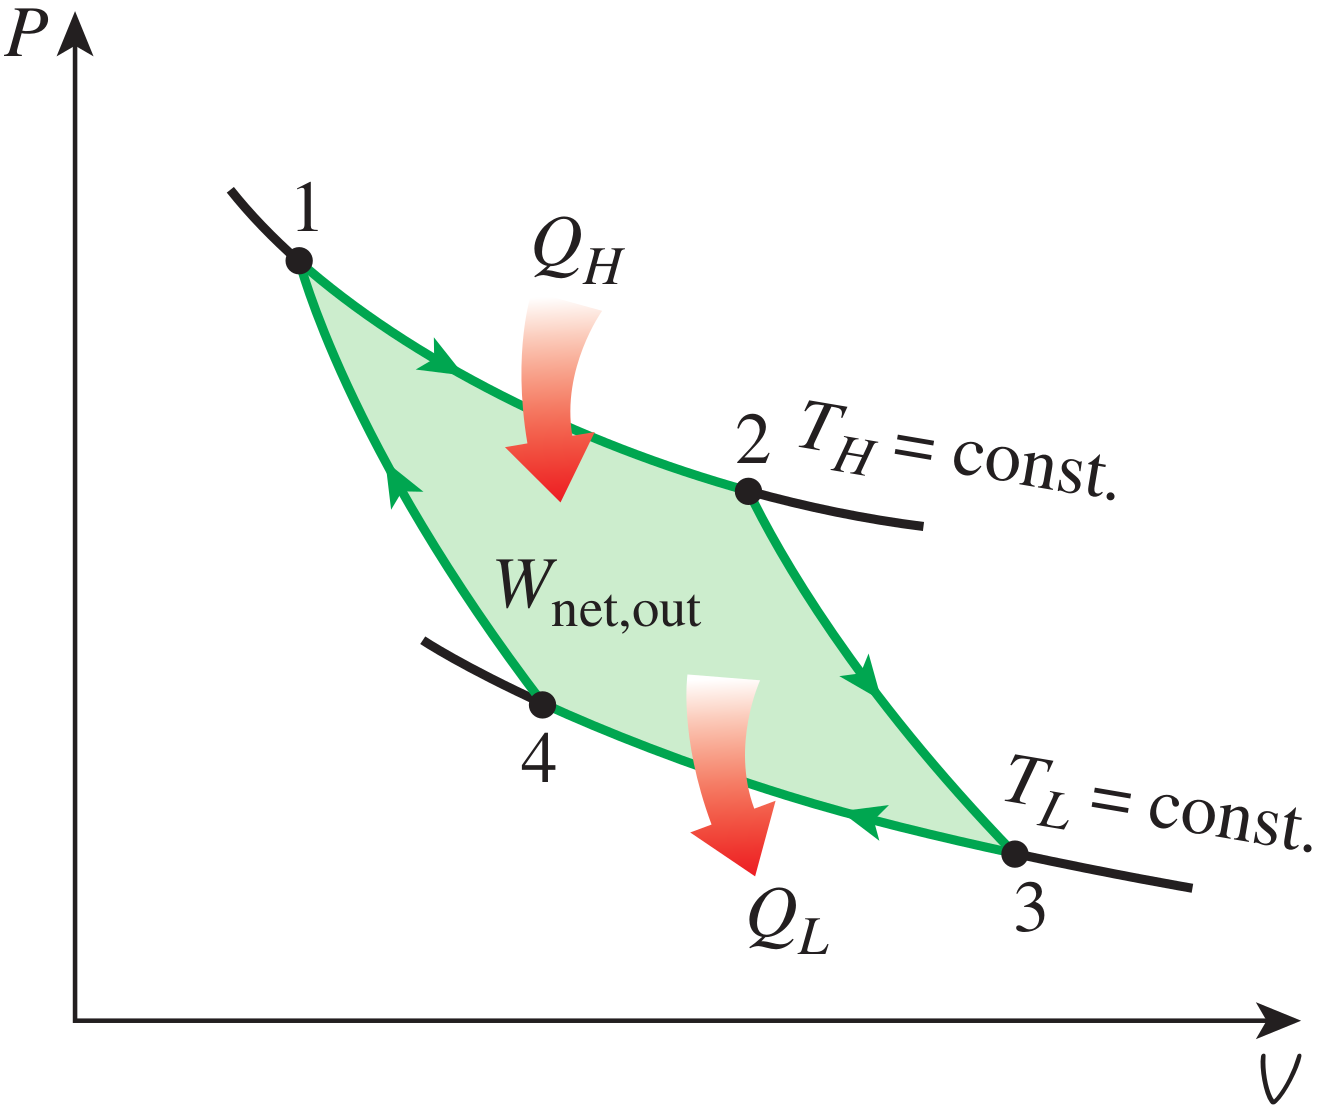
\includegraphics[width=0.5\textwidth]{Carnot_PV.png}
\caption{Carnot cycle - PV diagram \cite{2015}}
\label{fig:C2_CarnotPV}
\end{figure}

Using the first principle, the net work output is equal to $W_{net,out}=Q_H-Q_L$. This means that the efficiency of the cycle is given by
\begin{equation}
\setstretch{1}
\eta_{carnot} = \frac{W_{net,out}}{Q_H} = 1 - \frac{Q_H}{Q_L}
\end{equation} 
Considering that the working fluid is an ideal gas, it can be demonstrated that the heats $Q_H$ and $Q_L$ can be replaced by the corresponding temperature $T_H$ of the hot source and $T_C$ of the cold sink.
\begin{equation}
\setstretch{1}
\eta_{carnot}=1-\frac{T_H}{T_L}\label{eq:C2_eff_carnot}
\end{equation} 
The efficiency of the Carnot cycle is optimal. This implies that for any system playing with a hot source $T_H$ and a cold sink $T_C$, its efficiency cannot be greater than the Carnot efficiency with the \textbf{same} hot source and cold sink temperatures.
\subsection{Entropy}
\quad\, The last lines explained that a system with a hot source $T_H$ and a cold sink $T_C$ will never have a efficiency greater than the Carnot efficiency (for the same source and sink).

For such cycle, it has been demonstrated in 1865 by the German physician R. J. E. Clausius that "the cyclic integral $\oint\frac{\delta Q}{T}$ is always less than or equal to zero"\cite{2015}.
\begin{equation}
\setstretch{1}
\oint\frac{\delta Q}{T} = \frac{Q_H}{T_H} - \frac{Q_L}{T_L}\leq 0\label{eq:C2_cyc}
\end{equation}

For the Carnot cycle, the integral is equal to zeros because the two ratios $\frac{Q_H}{Q_L}$ and $\frac{T_H}{T_L}$ are equal.

From the definition \ref{eq:C2_cyc} can be defined a new state variable named \textbf{entropy}. The entropy S is always measured based on a reference point and, its expression is given in the relation (\ref{eq:C2_S}).
\begin{equation}
\setstretch{1}
dS \triangleq \frac{\delta Q_{rev}}{T}\label{eq:C2_S}
\end{equation}
where $\delta Q_{rev}$ is the "infinitesimal quantity of heat exchanged in a reversible way between the system and the environment at the temperature T"\cite{Dewallef2019}. 

For a reversible adiabatic transformation, the $\delta Q_{rev}=0$. This implies that the entropy remains constant. Such transformations are called \textbf{isentropic} transformation.

\subsection{Second principle definition}
\quad\, Defining the entropy gives a great tool to measure the "quality" of the transformation compared to a similar but reversible transformation.

Based on this definition, one formulation of the second principle of the thermodynamic is that for every transformation, the entropy of the final state of any isolated system is greater or equal to the one of the initial state.

Considering the system defined in the previous lines, it can be said that the increase of entropy $\Delta S_L$ of the cold sink have to be at least greater than the diminution of entropy $\Delta S_H$ of the hot source.

In the case of the Carnot cycle, both variations are equal. This is illustrated on the TS diagram \ref{fig:C2_CarnotTS} where the entropy of state \textbf{1} (resp. state \textbf{2}) is the same as the one of state \textbf{4} (resp. state \textbf{3}).
\begin{figure}[h]
\centering
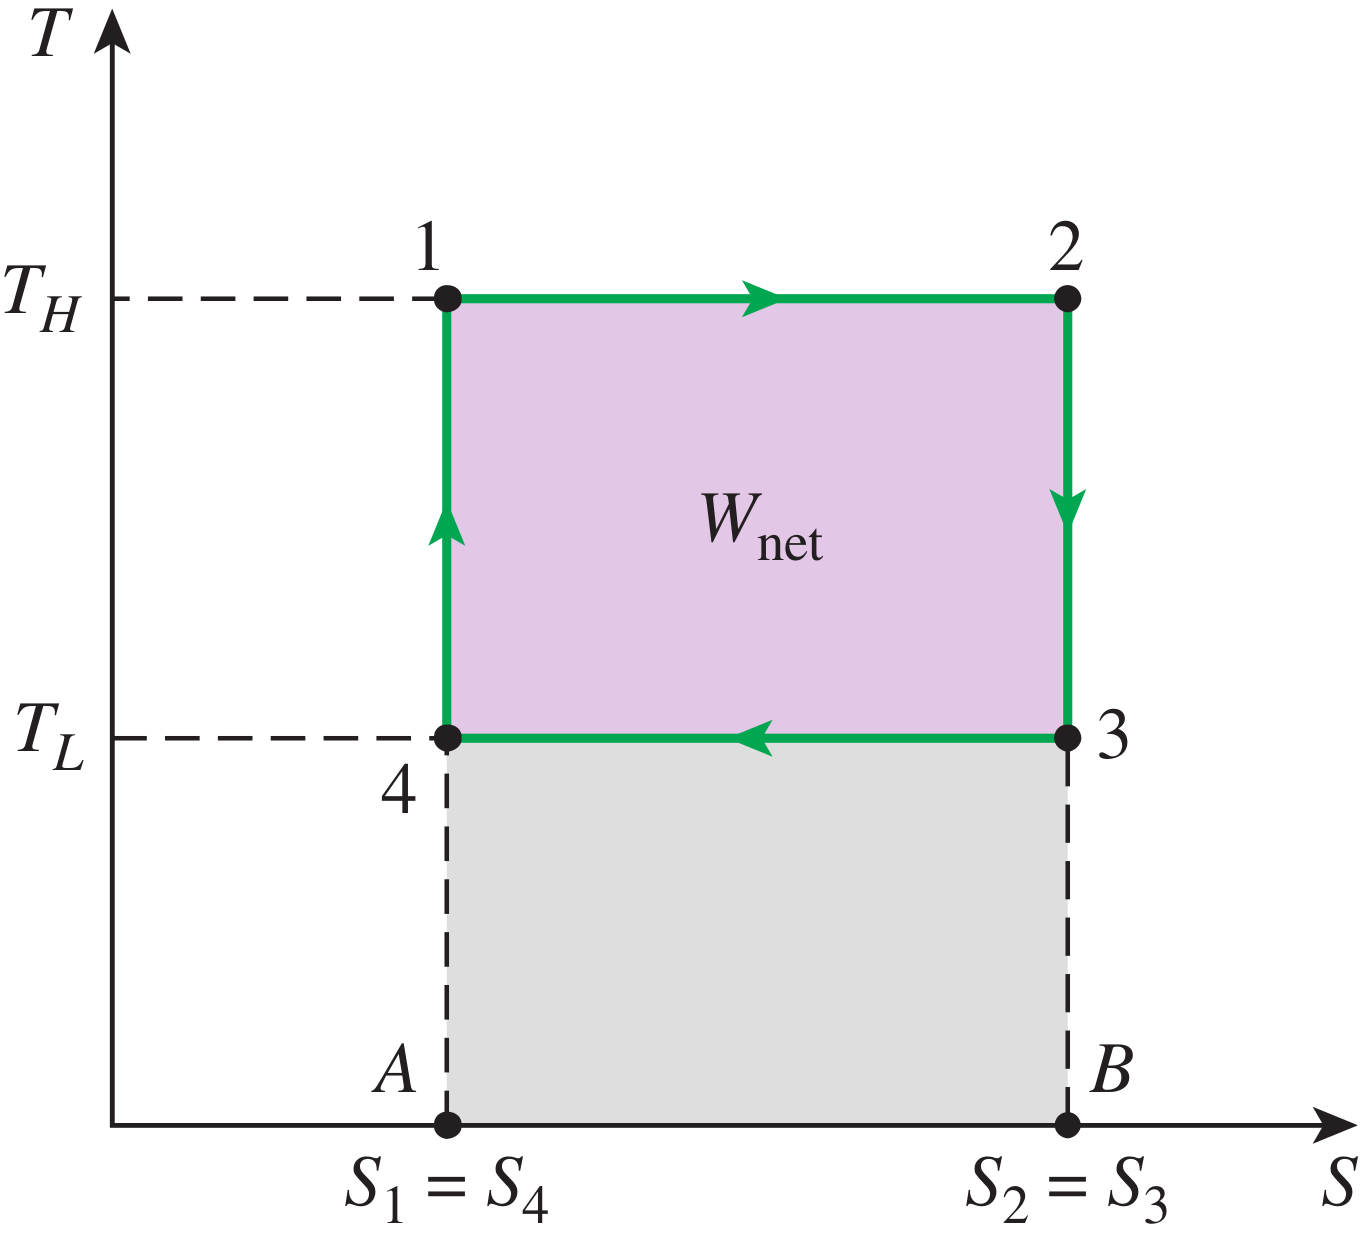
\includegraphics[width=0.5\textwidth]{Carnot_TS.png}
\caption{Carnot cycle - TS diagram \cite{2015}}
\label{fig:C2_CarnotTS}
\end{figure}

%\subsection{Exergy}
%\quad\, From now, it has not been clearly established a tool to establish the waste of energy when performing a transformation. It has been stated earlier that the "work done during a process depends on the initial state, the final state, and the process path. In the exergy analysis, the \textit{initial state} is specified [...], the process between the two states is executed in a \textit{reversible manner} [...], and the system must be in the \textit{dead state} at the end of the process"\cite{2015}. 
%
%The dead state is defined as being the state where the system is thermodynamic equilibrium with its immediate surrounding. This means that both will be at the same pressure and temperature and there is no unbalance (of any types) between the system and its surrounding. At this state, the system has zero exergy\citep{2015}.
%When the system arrived to such state, it cannot deliver any extra Joule of work. Indeed, supposing that there is a temperature gradient between the system and the immediate surrounding, it's possible to produce a work by "running a heat engine between these two temperature levels\citep{2015}.


\subsection{Computation of the thermodynamic properties}
\quad\, From now, the hypothesis of an ideal gas has been used for the computation of the previously established state variables. However, while this hypothesis remains quite valid when dealing with gas, it cannot be used for a real fluid (e.g. liquid water).

This problem can be solved using the Maxwell relations which provides a linked between the partial derivatives\footnote{For further information about partial derivative, see the annex \ref{annex_PD}} of the properties $p$, $v$, $T$ and $s$ for a simple compressible system \cite{2015}. 

Those relations can be derived from the four Gibbs relations expressed in (\ref{eq:C2_Gibbs}).

\begin{subequations}
\setstretch{1}
\begin{equation}
  du = Tds - Pdv \label{eq:C2_Gibbs1} 
\end{equation}    
\begin{equation}
  dh = Tds + vdP \label{eq:C2_Gibbs2} 
\end{equation}
\begin{equation}
  da = du - Tds - sdT = - Pdv - sdT \label{eq:C2_Gibbs3} 
\end{equation}    
\begin{equation}
  dg = dh - Tds - sdT = vdP - sdT \label{eq:C2_Gibbs4}
\end{equation} \label{eq:C2_Gibbs}
\end{subequations}

where the state variables $a$ and $g$ are the Helmholtz and Gibbs function (respectively).

Analyzing the relations allows to notice that each of them are of the form
\begin{align}
\setstretch{1}
dz &= Mdx + Ndy\label{eq:C2_Maxbase}\\
\text{with } \left.\frac{\partial M}{\partial y}\right|_x &= \left.\frac{\partial N}{\partial x}\right|_y\label{eq:C2_partMax}
\end{align}

Using this property, the links between the different state variables are easily obtained by applying the relation (\ref{eq:C2_partMax}) to the equations (\ref{eq:C2_Gibbs1}) to (\ref{eq:C2_Gibbs4}).
\begin{subequations}
\setstretch{1}
\begin{equation}
  \left.\frac{\partial T}{\partial v}\right|_s =  - \left.\frac{\partial p}{\partial s}\right|_v \label{eq:C2_Max1} 
\end{equation}    
\begin{equation}
  \left.\frac{\partial T}{\partial p}\right|_s = \left.\frac{\partial v}{\partial s}\right|_p \label{eq:C2_Max2}  
\end{equation}
\begin{equation}
  \left.\frac{\partial s}{\partial v}\right|_T = \left.\frac{\partial p}{\partial T}\right|_v \label{eq:C2_Max3} 
\end{equation}    
\begin{equation}
  \left.\frac{\partial s}{\partial p}\right|_T =  - \left.\frac{\partial v}{\partial T}\right|_p \label{eq:C2_Max4} 
\end{equation} \label{eq:C2_Max}
\end{subequations}

The relations (\ref{eq:C2_Max}) are called Maxwell equations are helpful in thermodynamics. They provide a method to calculate the variation of the entropy of a system based on the measurement of the variation of the pressure, volume and temperature.

However, this method for calculating the thermodynamic variables is limited to simple compressible system and cannot be used when the system involves "electrical, magnetic, and other effects"\cite{2015}.

These are the relations used when using a digital library for the thermodynamic assessment of the state of a pure fluid with real properties. The open-source library named \textbf{CoolProp}\cite{Bell2014} is one of the best known and. In this work, the library will be called many time when the ideal gas approximation is not relevant.

\subsection{Entropy variation}
\quad\, The previous subsection did introduce the four equations of state (\ref{eq:C2_Gibbs1}) to (\ref{eq:C2_Gibbs4}). Among those, the second equation allows to write the relation (\ref{eq:C2_ds})
\begin{equation}
ds = c_p\frac{dT}{T} - r\frac{dp}{p}\label{eq:C2_ds}
\end{equation}
using the definition (\ref{eq:C2_UP}) of the enthalpy variation and the \textbf{ideal gas equation} (\ref{eq:C2_GP}).

Performing the integration over the path of a transformation going from state \textbf{1} to state \textbf{2}, it can be obtained 
\begin{equation}
s_2 - s_1  = \int_1^2\frac{c_p}{T}dT - r\cdot ln\frac{p_2}{p_1}
\end{equation}
If it is supposed that the variation of the specific heat with respect to temperature are negligible, it can be written
\begin{equation}
s_2 - s_1= r\cdot \left(\frac{k}{k-1}\cdot ln\frac{T_2}{p_1} - ln\frac{p_2}{p_1}\right) = r\cdot ln\left[\frac{p_1}{p_2}\cdot\left(\frac{T_2}{T_1}\right)^\frac{k}{k-1}\right] \label{eq:C2_Deltas}
\end{equation}
where the $c_p=\frac{r\cdot k}{k-1}$ by using the two relations (\ref{eq:C2_r}) and (\ref{eq:C2_k}).

For an isentropic process, the equality $s_2=s_1$ is enforced. Thus, the following relationships can be derived.
\begin{subequations}
\setstretch{1}
\begin{equation}
\frac{p_2}{p_1} = \left(\frac{T_2}{T_1}\right)^\frac{k}{k-1}\label{eq:C2_isrelPT}
\end{equation}
\begin{equation}
\frac{\rho_2}{\rho_1} = \left(\frac{T_2}{T_1}\right)^\frac{1}{k-1}
\label{eq:C2_isrelrhoT}
\end{equation}
\label{eq:C2_isrel}
\end{subequations}

\subsection{Isentropic efficiency} \label{C2:Isen_eff}
\quad\, For any real transformations, the entropy \textbf{at the end state} is for the major number of cases greater that the one \textbf{at the beginning}. This means that the difference $s_2 - s_1$ is greater than zero.

This can be characterized by defining the isentropic efficiency as being the image of the irreversibilities induced by the transformation. this type of efficiency is very frequently used when studying the compression or the expansion of a fluid.

For a compression or an expansion, the isentropic efficiency is defined by stating that the pressure ratio $\frac{p_1}{p_2}$ is the identical for both the isentropic and non isentropic transformation. Let's substituting this ratio by the constant $\Pi$. 

Considering first the ideal case, the left equality in (\ref{eq:C2_isrel}) gives
\begin{equation}
T_{2,is} = T_1\cdot\Pi^\frac{k-1}{k}
\end{equation}
where the subscript says that the final state is at the same entropy that the starting state.

Then, for the real transformation, the left-hand-side of the relation (\ref{eq:C2_Deltas}) is greater than zero. This implies that
\begin{equation}
T_{2} > T_{2,is} = T_1\cdot\Pi^\frac{k-1}{k}
\end{equation}

As can be noticed, the real transformation leads to a final state temperature bigger than for the isentropic transformation. This difference allows to define the isentropic efficiency $\eta_{is}$. The definition varies based on the desired transformation
\begin{itemize}
\setstretch{1}
\item Compression: $\eta_{is}=\frac{T_{2,is}-T_1}{T_2-T_1}=\frac{h_{2,is}-h_1}{h_2-h_1}$
\item Expansion: $\eta_{is}=\frac{T_1-T_{2}}{T_1-T_{2,is}}=\frac{h_1-h_{2}}{h_1-h_{2,is}}$
\end{itemize}
where the temperature and the enthalpy variation provide the same output result due to the ideal gas hypothesis. For real fluid, the only valid definition of the isentropic efficiency is the one based on the enthalpy variation.

This conclude this second chapter related to the definition of the main thermodynamic notions. While these lines did not cover all the concepts, the minimum have been given to allows the description of the components integrated in the Brayton cycle. 

The next chapter will be devoted to the establishment of these descriptions. For each components, a state of the art and the definitions of the mains concepts will be provided. 
 %To summarize what have been done in this chapter, it has first been introduced the concept of open and closed system. Then, the notion of state variables has been defined. It has been exposed that these variables allows to assess the state of any closed or open system.
%
%Then, based on the two principles of the thermodynamic, it has been defined the notions of energy, enthalpy, specific heat and entropy. Those really valuable tools offer the means to fully determined the state of any systems. The energy conservation efficiency has been defined, providing a method to establish the quality of a transformation.
%
%The next chapter will be focused on the description of the different components constituting the Brayton cycle. The notions that have already been discussed in those lines will be supposed to be integrated by the reader. Therefore, those will not be repeated.
